\documentclass[twoside]{book}

% Packages required by doxygen
\usepackage{fixltx2e}
\usepackage{calc}
\usepackage{doxygen}
\usepackage[export]{adjustbox} % also loads graphicx
\usepackage{graphicx}
\usepackage[utf8]{inputenc}
\usepackage{makeidx}
\usepackage{multicol}
\usepackage{multirow}
\PassOptionsToPackage{warn}{textcomp}
\usepackage{textcomp}
\usepackage[nointegrals]{wasysym}
\usepackage[table]{xcolor}

% Font selection
\usepackage[T1]{fontenc}
\usepackage[scaled=.90]{helvet}
\usepackage{courier}
\usepackage{amssymb}
\usepackage{sectsty}
\renewcommand{\familydefault}{\sfdefault}
\allsectionsfont{%
  \fontseries{bc}\selectfont%
  \color{darkgray}%
}
\renewcommand{\DoxyLabelFont}{%
  \fontseries{bc}\selectfont%
  \color{darkgray}%
}
\newcommand{\+}{\discretionary{\mbox{\scriptsize$\hookleftarrow$}}{}{}}

% Page & text layout
\usepackage{geometry}
\geometry{%
  a4paper,%
  top=2.5cm,%
  bottom=2.5cm,%
  left=2.5cm,%
  right=2.5cm%
}
\tolerance=750
\hfuzz=15pt
\hbadness=750
\setlength{\emergencystretch}{15pt}
\setlength{\parindent}{0cm}
\setlength{\parskip}{3ex plus 2ex minus 2ex}
\makeatletter
\renewcommand{\paragraph}{%
  \@startsection{paragraph}{4}{0ex}{-1.0ex}{1.0ex}{%
    \normalfont\normalsize\bfseries\SS@parafont%
  }%
}
\renewcommand{\subparagraph}{%
  \@startsection{subparagraph}{5}{0ex}{-1.0ex}{1.0ex}{%
    \normalfont\normalsize\bfseries\SS@subparafont%
  }%
}
\makeatother

% Headers & footers
\usepackage{fancyhdr}
\pagestyle{fancyplain}
\fancyhead[LE]{\fancyplain{}{\bfseries\thepage}}
\fancyhead[CE]{\fancyplain{}{}}
\fancyhead[RE]{\fancyplain{}{\bfseries\leftmark}}
\fancyhead[LO]{\fancyplain{}{\bfseries\rightmark}}
\fancyhead[CO]{\fancyplain{}{}}
\fancyhead[RO]{\fancyplain{}{\bfseries\thepage}}
\fancyfoot[LE]{\fancyplain{}{}}
\fancyfoot[CE]{\fancyplain{}{}}
\fancyfoot[RE]{\fancyplain{}{\bfseries\scriptsize Generated by Doxygen }}
\fancyfoot[LO]{\fancyplain{}{\bfseries\scriptsize Generated by Doxygen }}
\fancyfoot[CO]{\fancyplain{}{}}
\fancyfoot[RO]{\fancyplain{}{}}
\renewcommand{\footrulewidth}{0.4pt}
\renewcommand{\chaptermark}[1]{%
  \markboth{#1}{}%
}
\renewcommand{\sectionmark}[1]{%
  \markright{\thesection\ #1}%
}

% Indices & bibliography
\usepackage{natbib}
\usepackage[titles]{tocloft}
\setcounter{tocdepth}{3}
\setcounter{secnumdepth}{5}
\makeindex

% Hyperlinks (required, but should be loaded last)
\usepackage{ifpdf}
\ifpdf
  \usepackage[pdftex,pagebackref=true]{hyperref}
\else
  \usepackage[ps2pdf,pagebackref=true]{hyperref}
\fi
\hypersetup{%
  colorlinks=true,%
  linkcolor=blue,%
  citecolor=blue,%
  unicode%
}

% Custom commands
\newcommand{\clearemptydoublepage}{%
  \newpage{\pagestyle{empty}\cleardoublepage}%
}

\usepackage{caption}
\captionsetup{labelsep=space,justification=centering,font={bf},singlelinecheck=off,skip=4pt,position=top}

%===== C O N T E N T S =====

\begin{document}

% Titlepage & ToC
\hypersetup{pageanchor=false,
             bookmarksnumbered=true,
             pdfencoding=unicode
            }
\pagenumbering{alph}
\begin{titlepage}
\vspace*{7cm}
\begin{center}%
{\Large A\+P\+C\+\_\+524 }\\
\vspace*{1cm}
{\large Generated by Doxygen 1.8.12}\\
\end{center}
\end{titlepage}
\clearemptydoublepage
\pagenumbering{roman}
\tableofcontents
\clearemptydoublepage
\pagenumbering{arabic}
\hypersetup{pageanchor=true}

%--- Begin generated contents ---
\chapter{Hierarchical Index}
\section{Class Hierarchy}
This inheritance list is sorted roughly, but not completely, alphabetically\+:\begin{DoxyCompactList}
\item \contentsline{section}{Domain}{\pageref{class_domain}}{}
\item \contentsline{section}{Field\+\_\+part}{\pageref{struct_field__part}}{}
\item \contentsline{section}{Grid}{\pageref{class_grid}}{}
\item \contentsline{section}{Input\+\_\+\+Info\+\_\+t}{\pageref{struct_input___info__t}}{}
\item \contentsline{section}{Interpolator}{\pageref{class_interpolator}}{}
\item \contentsline{section}{Particle}{\pageref{struct_particle}}{}
\item \contentsline{section}{Particle\+\_\+\+Compare}{\pageref{class_particle___compare}}{}
\item \contentsline{section}{Particle\+\_\+\+Field\+\_\+\+List}{\pageref{class_particle___field___list}}{}
\item \contentsline{section}{Pusher}{\pageref{class_pusher}}{}
\begin{DoxyCompactList}
\item \contentsline{section}{Boris}{\pageref{class_boris}}{}
\end{DoxyCompactList}
\end{DoxyCompactList}

\chapter{Class Index}
\section{Class List}
Here are the classes, structs, unions and interfaces with brief descriptions\+:\begin{DoxyCompactList}
\item\contentsline{section}{\hyperlink{class_boris}{Boris} }{\pageref{class_boris}}{}
\item\contentsline{section}{\hyperlink{class_domain}{Domain} }{\pageref{class_domain}}{}
\item\contentsline{section}{\hyperlink{struct_field__part}{Field\+\_\+part} }{\pageref{struct_field__part}}{}
\item\contentsline{section}{\hyperlink{class_grid}{Grid} \\*Class representing grid on which E and B fields and currents are defined }{\pageref{class_grid}}{}
\item\contentsline{section}{\hyperlink{struct_input___info__t}{Input\+\_\+\+Info\+\_\+t} }{\pageref{struct_input___info__t}}{}
\item\contentsline{section}{\hyperlink{struct_particle}{Particle} }{\pageref{struct_particle}}{}
\item\contentsline{section}{\hyperlink{class_particle___compare}{Particle\+\_\+\+Compare} }{\pageref{class_particle___compare}}{}
\item\contentsline{section}{\hyperlink{class_particle___field___list}{Particle\+\_\+\+Field\+\_\+\+List} }{\pageref{class_particle___field___list}}{}
\item\contentsline{section}{\hyperlink{class_pusher}{Pusher} }{\pageref{class_pusher}}{}
\end{DoxyCompactList}

\chapter{Class Documentation}
\hypertarget{class_boris}{}\section{Boris Class Reference}
\label{class_boris}\index{Boris@{Boris}}


Inheritance diagram for Boris\+:\nopagebreak
\begin{figure}[H]
\begin{center}
\leavevmode
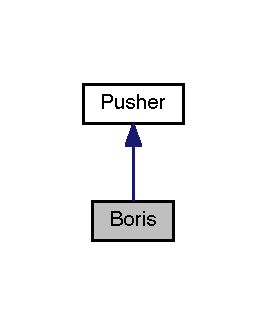
\includegraphics[width=128pt]{class_boris__inherit__graph}
\end{center}
\end{figure}


Collaboration diagram for Boris\+:\nopagebreak
\begin{figure}[H]
\begin{center}
\leavevmode
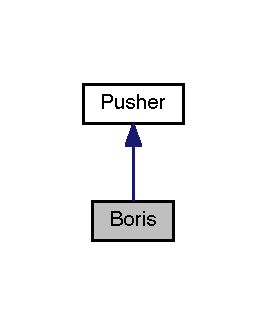
\includegraphics[width=128pt]{class_boris__coll__graph}
\end{center}
\end{figure}
\subsection*{Public Member Functions}
\begin{DoxyCompactItemize}
\item 
\hypertarget{class_boris_a1cf5027803211109530e12ddd434ef5c}{}\label{class_boris_a1cf5027803211109530e12ddd434ef5c} 
int {\bfseries Step} (\hyperlink{struct_particle}{Particle} $\ast$part, \hyperlink{struct_field__part}{Field\+\_\+part} $\ast$field, double dt)
\end{DoxyCompactItemize}


The documentation for this class was generated from the following files\+:\begin{DoxyCompactItemize}
\item 
src/pusher/boris.\+hpp\item 
src/pusher/boris.\+cpp\end{DoxyCompactItemize}

\hypertarget{class_domain}{}\section{Domain Class Reference}
\label{class_domain}\index{Domain@{Domain}}
\subsection*{Public Member Functions}
\begin{DoxyCompactItemize}
\item 
\hypertarget{class_domain_a27d315196d4c79b6e80c2123bc06c975}{}\label{class_domain_a27d315196d4c79b6e80c2123bc06c975} 
{\bfseries Domain} (int size, int rank, \hyperlink{struct_input___info__t}{Input\+\_\+\+Info\+\_\+t} $\ast$input\+\_\+info)
\item 
\hypertarget{class_domain_ac1b8746a797f7ab2123999f8ea06a9dc}{}\label{class_domain_ac1b8746a797f7ab2123999f8ea06a9dc} 
int {\bfseries getn\+Ghosts} (void)
\item 
\hypertarget{class_domain_a618e79f2f494218923d40cf014997b69}{}\label{class_domain_a618e79f2f494218923d40cf014997b69} 
int $\ast$ {\bfseries getnxyz} (void)
\item 
\hypertarget{class_domain_a603724205a08d6f17755d4d2152209f0}{}\label{class_domain_a603724205a08d6f17755d4d2152209f0} 
double $\ast$ {\bfseries getxyz0} (void)
\item 
\hypertarget{class_domain_a85f15ae00a318da34e8dfde4e0f1fdab}{}\label{class_domain_a85f15ae00a318da34e8dfde4e0f1fdab} 
double $\ast$ {\bfseries get\+Lxyz} (void)
\end{DoxyCompactItemize}


The documentation for this class was generated from the following files\+:\begin{DoxyCompactItemize}
\item 
src/domain/domain.\+hpp\item 
src/domain/domain.\+cpp\end{DoxyCompactItemize}

\hypertarget{struct_field__part}{}\section{Field\+\_\+part Struct Reference}
\label{struct_field__part}\index{Field\+\_\+part@{Field\+\_\+part}}
\subsection*{Public Attributes}
\begin{DoxyCompactItemize}
\item 
\hypertarget{struct_field__part_a88cbf49b8585552707cc4d2b4fb72745}{}\label{struct_field__part_a88cbf49b8585552707cc4d2b4fb72745} 
double {\bfseries e1}
\item 
\hypertarget{struct_field__part_ae956ea9079af38e4eaafb7b00f317ce9}{}\label{struct_field__part_ae956ea9079af38e4eaafb7b00f317ce9} 
double {\bfseries e2}
\item 
\hypertarget{struct_field__part_a6a892083caadc7e684af6bdc9e0e4cb9}{}\label{struct_field__part_a6a892083caadc7e684af6bdc9e0e4cb9} 
double {\bfseries e3}
\item 
\hypertarget{struct_field__part_a3d9f01728f0f1ce0a706e55186680734}{}\label{struct_field__part_a3d9f01728f0f1ce0a706e55186680734} 
double {\bfseries b1}
\item 
\hypertarget{struct_field__part_a0758e5f57a7a07d325a0ac477a263da6}{}\label{struct_field__part_a0758e5f57a7a07d325a0ac477a263da6} 
double {\bfseries b2}
\item 
\hypertarget{struct_field__part_a72a1f1e86c0a26aae9b01fc827c8852f}{}\label{struct_field__part_a72a1f1e86c0a26aae9b01fc827c8852f} 
double {\bfseries b3}
\end{DoxyCompactItemize}


The documentation for this struct was generated from the following file\+:\begin{DoxyCompactItemize}
\item 
src/particles/particle.\+hpp\end{DoxyCompactItemize}

\hypertarget{class_grid}{}\section{Grid Class Reference}
\label{class_grid}\index{Grid@{Grid}}


Class representing grid on which E and B fields and currents are defined.  




{\ttfamily \#include $<$grid.\+hpp$>$}

\subsection*{Public Member Functions}
\begin{DoxyCompactItemize}
\item 
\hypertarget{class_grid_a696a4b0b7335bed4b9b712e72eb1034e}{}\label{class_grid_a696a4b0b7335bed4b9b712e72eb1034e} 
{\bfseries Grid} (int $\ast$nxyz, int n\+Ghosts, double $\ast$xyz0, double $\ast$Lxyz)
\item 
int \hyperlink{class_grid_ab1cc80fe3a856f09d59b51ef558764c3}{evolve\+Fields} (double dt)
\begin{DoxyCompactList}\small\item\em Evolve Electric and Magnetic fields in time. \end{DoxyCompactList}\item 
int \hyperlink{class_grid_a93ea3ff4d2e7bdc9b5c4cbe9fe604f76}{get\+Field\+Interpolator\+Vec} (int cell\+ID, double $\ast$Interpolator\+Vec)
\begin{DoxyCompactList}\small\item\em Return vector for field interpolation. \end{DoxyCompactList}\item 
int \hyperlink{class_grid_a7347c885ddb7abbcc9390b6fec4ba42b}{get\+Cell\+ID} (double x, double y, double z)
\begin{DoxyCompactList}\small\item\em Get cell ID based on particle position. \end{DoxyCompactList}\item 
\hypertarget{class_grid_a2bf56b3564559d4ac6533ee5610dc2ca}{}\label{class_grid_a2bf56b3564559d4ac6533ee5610dc2ca} 
int \hyperlink{class_grid_a2bf56b3564559d4ac6533ee5610dc2ca}{get\+Number\+Of\+Cells} ()
\begin{DoxyCompactList}\small\item\em Get total number of cells. \end{DoxyCompactList}\item 
double \hyperlink{class_grid_a7c37daac383190622c7cf37597101510}{get\+Step\+Size} (int dimension)
\begin{DoxyCompactList}\small\item\em Get number of cells along dimension in grid. \end{DoxyCompactList}\item 
\hypertarget{class_grid_ae677a62490f6c432895e2ac38e9c0ef8}{}\label{class_grid_ae677a62490f6c432895e2ac38e9c0ef8} 
void {\bfseries update\+Ghost\+Cells} ()
\item 
\hypertarget{class_grid_a3ec170bd98cf658e567ac0d6a4975ceb}{}\label{class_grid_a3ec170bd98cf658e567ac0d6a4975ceb} 
int {\bfseries get\+Ghost\+Vec\+Size} ()
\item 
\hypertarget{class_grid_a768ae91746ecfc1d7b9172c431ecf45c}{}\label{class_grid_a768ae91746ecfc1d7b9172c431ecf45c} 
void {\bfseries get\+Ghost\+Vec} (const int side, double $\ast$ghost\+Vec)
\item 
\hypertarget{class_grid_a606fe5333db63f24d270a0546608f1f4}{}\label{class_grid_a606fe5333db63f24d270a0546608f1f4} 
void {\bfseries get\+Ghost\+Vec\+Alt} (const int side, double $\ast$ghost\+Vec)
\item 
\hypertarget{class_grid_aa24065a7d9fedd06cdb78a4c81c44b79}{}\label{class_grid_aa24065a7d9fedd06cdb78a4c81c44b79} 
void {\bfseries set\+Ghost\+Vec} (const int side, const double $\ast$ghost\+Vec)
\item 
\hypertarget{class_grid_a5d47f8db0c280c26467b5a91465b7d40}{}\label{class_grid_a5d47f8db0c280c26467b5a91465b7d40} 
void {\bfseries set\+Ghost\+Vec\+Alt} (const int side, const double $\ast$ghost\+Vec)
\end{DoxyCompactItemize}
\subsection*{Protected Member Functions}
\begin{DoxyCompactItemize}
\item 
\hypertarget{class_grid_a23877f79f95e9a109e908d930c8036b4}{}\label{class_grid_a23877f79f95e9a109e908d930c8036b4} 
double $\ast$$\ast$$\ast$ {\bfseries new\+Field\+\_\+} ()
\item 
\hypertarget{class_grid_acaa1c3843fd96478b3a5e9f62401d8e0}{}\label{class_grid_acaa1c3843fd96478b3a5e9f62401d8e0} 
void {\bfseries delete\+Field\+\_\+} (double $\ast$$\ast$$\ast$field\+Pt)
\item 
\hypertarget{class_grid_a91fc198085fdfeaa6378a99db4dbc6ac}{}\label{class_grid_a91fc198085fdfeaa6378a99db4dbc6ac} 
int {\bfseries side\+To\+Index\+\_\+} (const int side)
\item 
\hypertarget{class_grid_af631b4ec77d5ad46d17abe24155114c1}{}\label{class_grid_af631b4ec77d5ad46d17abe24155114c1} 
void {\bfseries check\+Input\+\_\+} ()
\item 
\hypertarget{class_grid_adfae48e6068488739c8823bc575f4f0a}{}\label{class_grid_adfae48e6068488739c8823bc575f4f0a} 
void {\bfseries slice\+Mat\+To\+Vec\+\_\+} (double $\ast$$\ast$$\ast$const mat, const int side)
\item 
\hypertarget{class_grid_a99b9c649ef28f41fa939d4517f504eb0}{}\label{class_grid_a99b9c649ef28f41fa939d4517f504eb0} 
void {\bfseries unslice\+Mat\+To\+Vec\+\_\+} (double $\ast$$\ast$$\ast$mat, const int side)
\end{DoxyCompactItemize}
\subsection*{Protected Attributes}
\begin{DoxyCompactItemize}
\item 
\hypertarget{class_grid_af1915aaf156bbc0677d2f8853643fddb}{}\label{class_grid_af1915aaf156bbc0677d2f8853643fddb} 
const int {\bfseries nx\+\_\+}
\item 
\hypertarget{class_grid_a017c2ce200149e3f6b9e1feec7432be3}{}\label{class_grid_a017c2ce200149e3f6b9e1feec7432be3} 
const int {\bfseries ny\+\_\+}
\item 
\hypertarget{class_grid_af66fb5b609dbae6a5c47db6a3726a109}{}\label{class_grid_af66fb5b609dbae6a5c47db6a3726a109} 
const int {\bfseries nz\+\_\+}
\item 
\hypertarget{class_grid_a98debafd3794f12c96db014d5a81eaba}{}\label{class_grid_a98debafd3794f12c96db014d5a81eaba} 
const int {\bfseries n\+Ghosts\+\_\+}
\item 
\hypertarget{class_grid_aace2e7b11d2a22c87ea16b532e6c20a4}{}\label{class_grid_aace2e7b11d2a22c87ea16b532e6c20a4} 
const double {\bfseries x0\+\_\+}
\item 
\hypertarget{class_grid_a68796bd5f9418d0777516b19871a77bd}{}\label{class_grid_a68796bd5f9418d0777516b19871a77bd} 
const double {\bfseries y0\+\_\+}
\item 
\hypertarget{class_grid_a6532d09f92dfa370d11e302a6a3eff9a}{}\label{class_grid_a6532d09f92dfa370d11e302a6a3eff9a} 
const double {\bfseries z0\+\_\+}
\item 
\hypertarget{class_grid_a2ee01f81fd767620cfcae164be951713}{}\label{class_grid_a2ee01f81fd767620cfcae164be951713} 
const double {\bfseries Lx\+\_\+}
\item 
\hypertarget{class_grid_a7cd0a2a18b5f0d063984da365de2d893}{}\label{class_grid_a7cd0a2a18b5f0d063984da365de2d893} 
const double {\bfseries Ly\+\_\+}
\item 
\hypertarget{class_grid_afb8df0a51563cb751ccd94cc29b69e7a}{}\label{class_grid_afb8df0a51563cb751ccd94cc29b69e7a} 
const double {\bfseries Lz\+\_\+}
\item 
\hypertarget{class_grid_a168dc221b038fa0130606ddba9281534}{}\label{class_grid_a168dc221b038fa0130606ddba9281534} 
const int {\bfseries i\+Beg\+\_\+}
\item 
\hypertarget{class_grid_ac7599170601ea6b6d1a7d6c4b671b24c}{}\label{class_grid_ac7599170601ea6b6d1a7d6c4b671b24c} 
const int {\bfseries j\+Beg\+\_\+}
\item 
\hypertarget{class_grid_a9a3b3086af10cf5e3e3d9136e8082d3b}{}\label{class_grid_a9a3b3086af10cf5e3e3d9136e8082d3b} 
const int {\bfseries k\+Beg\+\_\+}
\item 
\hypertarget{class_grid_a5a93654972769d0c6167501b72e47a8a}{}\label{class_grid_a5a93654972769d0c6167501b72e47a8a} 
const int {\bfseries i\+End\+\_\+}
\item 
\hypertarget{class_grid_ab7f65f3bf13b95fff3f0d2317078a185}{}\label{class_grid_ab7f65f3bf13b95fff3f0d2317078a185} 
const int {\bfseries j\+End\+\_\+}
\item 
\hypertarget{class_grid_af73398f1f22f32beb71081b33eb7aa88}{}\label{class_grid_af73398f1f22f32beb71081b33eb7aa88} 
const int {\bfseries k\+End\+\_\+}
\item 
\hypertarget{class_grid_a63a64dc2ea909ee51cd0a4cd00a3fb11}{}\label{class_grid_a63a64dc2ea909ee51cd0a4cd00a3fb11} 
const double {\bfseries dx\+\_\+}
\item 
\hypertarget{class_grid_a210cf6638f34de1854c4430905d44401}{}\label{class_grid_a210cf6638f34de1854c4430905d44401} 
const double {\bfseries dy\+\_\+}
\item 
\hypertarget{class_grid_a88975e0c193ba200d3bb20d1b7f5aa08}{}\label{class_grid_a88975e0c193ba200d3bb20d1b7f5aa08} 
const double {\bfseries dz\+\_\+}
\item 
\hypertarget{class_grid_a2ca6e799692e4196f745402785c38eea}{}\label{class_grid_a2ca6e799692e4196f745402785c38eea} 
const double {\bfseries idx\+\_\+}
\item 
\hypertarget{class_grid_ae03d8f59e2a2b45691746c36c6dd3e90}{}\label{class_grid_ae03d8f59e2a2b45691746c36c6dd3e90} 
const double {\bfseries idy\+\_\+}
\item 
\hypertarget{class_grid_aa7bbf073678332ff181b08c9e1d893e5}{}\label{class_grid_aa7bbf073678332ff181b08c9e1d893e5} 
const double {\bfseries idz\+\_\+}
\item 
\hypertarget{class_grid_a873f5a0ef0ef52b485a3b38237c3e916}{}\label{class_grid_a873f5a0ef0ef52b485a3b38237c3e916} 
const int {\bfseries n\+Real\+Pts\+Y\+Z\+Plane\+\_\+}
\item 
\hypertarget{class_grid_a2bae6b711883328cddf69d37af10732c}{}\label{class_grid_a2bae6b711883328cddf69d37af10732c} 
const int {\bfseries n\+Fields\+\_\+}
\item 
\hypertarget{class_grid_a4c757d84f22696e88a4c500e35742ee2}{}\label{class_grid_a4c757d84f22696e88a4c500e35742ee2} 
const int {\bfseries ghost\+Vec\+Size\+\_\+}
\item 
\hypertarget{class_grid_a4f82b7703c89f4d202a636b77619cc4f}{}\label{class_grid_a4f82b7703c89f4d202a636b77619cc4f} 
double $\ast$$\ast$$\ast$ {\bfseries Ex\+\_\+}
\item 
\hypertarget{class_grid_a29021cc53090316898144ee2987b3b3f}{}\label{class_grid_a29021cc53090316898144ee2987b3b3f} 
double $\ast$$\ast$$\ast$ {\bfseries Ey\+\_\+}
\item 
\hypertarget{class_grid_ae258f0a77f3324405298f756c44995d6}{}\label{class_grid_ae258f0a77f3324405298f756c44995d6} 
double $\ast$$\ast$$\ast$ {\bfseries Ez\+\_\+}
\item 
\hypertarget{class_grid_af3e410cb198880388039e4a49a9bc55d}{}\label{class_grid_af3e410cb198880388039e4a49a9bc55d} 
double $\ast$$\ast$$\ast$ {\bfseries Bx\+\_\+}
\item 
\hypertarget{class_grid_acbb9cb3b41fbff9958955e92a42efe58}{}\label{class_grid_acbb9cb3b41fbff9958955e92a42efe58} 
double $\ast$$\ast$$\ast$ {\bfseries By\+\_\+}
\item 
\hypertarget{class_grid_ad2cec062b407c6ac77d5aac144c71258}{}\label{class_grid_ad2cec062b407c6ac77d5aac144c71258} 
double $\ast$$\ast$$\ast$ {\bfseries Bz\+\_\+}
\item 
\hypertarget{class_grid_a5310eeec619f3f8ec782fd3a1757d29e}{}\label{class_grid_a5310eeec619f3f8ec782fd3a1757d29e} 
double $\ast$$\ast$$\ast$ {\bfseries Bx\+\_\+tm1\+\_\+}
\item 
\hypertarget{class_grid_a8febeb882155e2d76b15d4279c52698d}{}\label{class_grid_a8febeb882155e2d76b15d4279c52698d} 
double $\ast$$\ast$$\ast$ {\bfseries By\+\_\+tm1\+\_\+}
\item 
\hypertarget{class_grid_a90815801f8c229cfd47da1566b36e57d}{}\label{class_grid_a90815801f8c229cfd47da1566b36e57d} 
double $\ast$$\ast$$\ast$ {\bfseries Bz\+\_\+tm1\+\_\+}
\item 
\hypertarget{class_grid_a8d4ca4b13f4d3963bd8e78c48e527fc8}{}\label{class_grid_a8d4ca4b13f4d3963bd8e78c48e527fc8} 
double $\ast$$\ast$$\ast$ {\bfseries Jx\+\_\+}
\item 
\hypertarget{class_grid_a320132efacf9d773c82a97c2f838cb06}{}\label{class_grid_a320132efacf9d773c82a97c2f838cb06} 
double $\ast$$\ast$$\ast$ {\bfseries Jy\+\_\+}
\item 
\hypertarget{class_grid_ade5d55b0ce8f87a22ce8bf18047486a4}{}\label{class_grid_ade5d55b0ce8f87a22ce8bf18047486a4} 
double $\ast$$\ast$$\ast$ {\bfseries Jz\+\_\+}
\item 
\hypertarget{class_grid_a5dcd38dc5d89c1a2a22af25b34998a63}{}\label{class_grid_a5dcd38dc5d89c1a2a22af25b34998a63} 
double $\ast$ {\bfseries slice\+Tmp\+\_\+}
\end{DoxyCompactItemize}


\subsection{Detailed Description}
Class representing grid on which E and B fields and currents are defined. 

\hyperlink{class_grid}{Grid} has ghost cells on each face. The ghost cell updating in y and z arises from periodic boundary conditions. x-\/direction ghost cells allow communication between M\+PI domains.

Following Yee (1966), electric fields and currents reside on edges, and magnetic fields on faces. Fields are updated using a set of finite-\/difference equations approximating Ampere\textquotesingle{}s and Faraday\textquotesingle{}s Laws.

A set of getters are available to allow particles to interpolate electric fields based on their position. 

\subsection{Member Function Documentation}
\hypertarget{class_grid_ab1cc80fe3a856f09d59b51ef558764c3}{}\label{class_grid_ab1cc80fe3a856f09d59b51ef558764c3} 
\index{Grid@{Grid}!evolve\+Fields@{evolve\+Fields}}
\index{evolve\+Fields@{evolve\+Fields}!Grid@{Grid}}
\subsubsection{\texorpdfstring{evolve\+Fields()}{evolveFields()}}
{\footnotesize\ttfamily int Grid\+::evolve\+Fields (\begin{DoxyParamCaption}\item[{double}]{dt }\end{DoxyParamCaption})}



Evolve Electric and Magnetic fields in time. 

Uses Yee algorithm to advance E and B fields. \hypertarget{class_grid_a7347c885ddb7abbcc9390b6fec4ba42b}{}\label{class_grid_a7347c885ddb7abbcc9390b6fec4ba42b} 
\index{Grid@{Grid}!get\+Cell\+ID@{get\+Cell\+ID}}
\index{get\+Cell\+ID@{get\+Cell\+ID}!Grid@{Grid}}
\subsubsection{\texorpdfstring{get\+Cell\+I\+D()}{getCellID()}}
{\footnotesize\ttfamily int Grid\+::get\+Cell\+ID (\begin{DoxyParamCaption}\item[{double}]{x,  }\item[{double}]{y,  }\item[{double}]{z }\end{DoxyParamCaption})}



Get cell ID based on particle position. 

Cell ID is uniquely given by (ny\+\_\+$\ast$nz\+\_\+)$\ast$ix + nz\+\_\+$\ast$iy + iz. Returns -\/1 if particle is not on grid. \hypertarget{class_grid_a93ea3ff4d2e7bdc9b5c4cbe9fe604f76}{}\label{class_grid_a93ea3ff4d2e7bdc9b5c4cbe9fe604f76} 
\index{Grid@{Grid}!get\+Field\+Interpolator\+Vec@{get\+Field\+Interpolator\+Vec}}
\index{get\+Field\+Interpolator\+Vec@{get\+Field\+Interpolator\+Vec}!Grid@{Grid}}
\subsubsection{\texorpdfstring{get\+Field\+Interpolator\+Vec()}{getFieldInterpolatorVec()}}
{\footnotesize\ttfamily int Grid\+::get\+Field\+Interpolator\+Vec (\begin{DoxyParamCaption}\item[{int}]{cell\+ID,  }\item[{double $\ast$}]{Interpolator\+Vec }\end{DoxyParamCaption})}



Return vector for field interpolation. 

Based on cell\+ID, return relevant edge E and face B fields and cell origin, in format \mbox{[}x, y, z, ... Ex( ix, iy, iz ), Ex( ix, iy+1,iz ), Ex( ix, iy+1, iz+1 ), Ex( ix, iy, iz+1 ), ... Ey( ix, iy, iz ), Ey( ix, iy, iz+1 ), Ey( ix+1, iy, iz+1 ), Ey( ix+1, iy, iz ), ... Ez( ix, iy, iz ), Ez( ix+1, iy, iz ), Ez( ix+1, iy+1, iz ), Ez( ix, iy+1, iz ), ... Bx( ix, iy, iz ), Bx( ix+1, iy, iz ), ... By( ix, iy, iz ), By( ix, iy+1, iz ), ... Bz( ix, iy, iz ), Bz( ix, iy, iz+1 ), ...\mbox{]} where ix, iy, and iz are the row indices for each of the three dimensions (calculated from the cell\+ID) \hypertarget{class_grid_a7c37daac383190622c7cf37597101510}{}\label{class_grid_a7c37daac383190622c7cf37597101510} 
\index{Grid@{Grid}!get\+Step\+Size@{get\+Step\+Size}}
\index{get\+Step\+Size@{get\+Step\+Size}!Grid@{Grid}}
\subsubsection{\texorpdfstring{get\+Step\+Size()}{getStepSize()}}
{\footnotesize\ttfamily double Grid\+::get\+Step\+Size (\begin{DoxyParamCaption}\item[{int}]{dimension }\end{DoxyParamCaption})}



Get number of cells along dimension in grid. 

Returns number of cells along dimension according to; dimension = 0\+: x dimension = 1\+: y dimension = 2\+: z Returns -\/1 if invalid dimension. 

The documentation for this class was generated from the following files\+:\begin{DoxyCompactItemize}
\item 
src/grid/grid.\+hpp\item 
src/grid/grid.\+cpp\item 
src/grid/o\+Grid.\+cpp\item 
src/grid/spooky\+Grid.\+cpp\end{DoxyCompactItemize}

\hypertarget{struct_input___info__t}{}\section{Input\+\_\+\+Info\+\_\+t Struct Reference}
\label{struct_input___info__t}\index{Input\+\_\+\+Info\+\_\+t@{Input\+\_\+\+Info\+\_\+t}}
\subsection*{Public Attributes}
\begin{DoxyCompactItemize}
\item 
\hypertarget{struct_input___info__t_a5feb8e378b6fbd9381ed57ef740442c9}{}\label{struct_input___info__t_a5feb8e378b6fbd9381ed57ef740442c9} 
int {\bfseries nx}
\item 
\hypertarget{struct_input___info__t_a3acc90c9a977cd1c634b574df77e0f60}{}\label{struct_input___info__t_a3acc90c9a977cd1c634b574df77e0f60} 
long {\bfseries np}
\item 
\hypertarget{struct_input___info__t_aaa9358b4befa5b3d1e49ad5e01e1479a}{}\label{struct_input___info__t_aaa9358b4befa5b3d1e49ad5e01e1479a} 
int {\bfseries nt}
\item 
\hypertarget{struct_input___info__t_a455e1f52527a77caf01262001159bc24}{}\label{struct_input___info__t_a455e1f52527a77caf01262001159bc24} 
int {\bfseries restart}
\item 
\hypertarget{struct_input___info__t_ab546d417babbd8d41c67a68d46100a91}{}\label{struct_input___info__t_ab546d417babbd8d41c67a68d46100a91} 
double {\bfseries dens}
\item 
\hypertarget{struct_input___info__t_ab3e5d89692bbc8eb2b14a22cad1e790a}{}\label{struct_input___info__t_ab3e5d89692bbc8eb2b14a22cad1e790a} 
double {\bfseries temp}
\end{DoxyCompactItemize}


The documentation for this struct was generated from the following file\+:\begin{DoxyCompactItemize}
\item 
src/\+I\+O/I\+O.\+hpp\end{DoxyCompactItemize}

\hypertarget{struct_particle}{}\section{Particle Struct Reference}
\label{struct_particle}\index{Particle@{Particle}}


Collaboration diagram for Particle\+:
\nopagebreak
\begin{figure}[H]
\begin{center}
\leavevmode
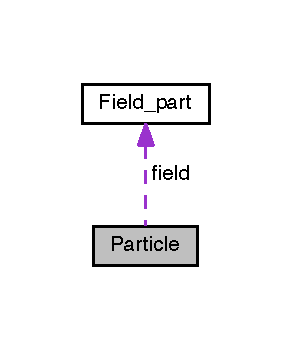
\includegraphics[width=140pt]{struct_particle__coll__graph}
\end{center}
\end{figure}
\subsection*{Public Attributes}
\begin{DoxyCompactItemize}
\item 
\hypertarget{struct_particle_ad565762c5789038a38b77b8b7b73108e}{}\label{struct_particle_ad565762c5789038a38b77b8b7b73108e} 
double {\bfseries x1}
\item 
\hypertarget{struct_particle_a4c6d32080244942982cddb6c6908ee5d}{}\label{struct_particle_a4c6d32080244942982cddb6c6908ee5d} 
double {\bfseries x2}
\item 
\hypertarget{struct_particle_a252ebc476e3bdf3deb799de97b55c136}{}\label{struct_particle_a252ebc476e3bdf3deb799de97b55c136} 
double {\bfseries x3}
\item 
\hypertarget{struct_particle_a50d359033a629a9004251ae121f104a3}{}\label{struct_particle_a50d359033a629a9004251ae121f104a3} 
double {\bfseries v1}
\item 
\hypertarget{struct_particle_afbd6500ae530cee3449acea407196faa}{}\label{struct_particle_afbd6500ae530cee3449acea407196faa} 
double {\bfseries v2}
\item 
\hypertarget{struct_particle_a70a3e519b0d00c7a34c7bcd8ad3f0934}{}\label{struct_particle_a70a3e519b0d00c7a34c7bcd8ad3f0934} 
double {\bfseries v3}
\item 
\hypertarget{struct_particle_a566dcc1de4bdc01251776948798ea8e1}{}\label{struct_particle_a566dcc1de4bdc01251776948798ea8e1} 
double {\bfseries q}
\item 
\hypertarget{struct_particle_aedcc7e1bc53b0e2b1a4a07c9a1b47563}{}\label{struct_particle_aedcc7e1bc53b0e2b1a4a07c9a1b47563} 
double {\bfseries m}
\item 
\hypertarget{struct_particle_a8c5aa296be47df7d6bbfe3a3f602f3d5}{}\label{struct_particle_a8c5aa296be47df7d6bbfe3a3f602f3d5} 
int {\bfseries my\+\_\+id}
\item 
\hypertarget{struct_particle_a2e15a24415109ae666abf197c6c0e7f8}{}\label{struct_particle_a2e15a24415109ae666abf197c6c0e7f8} 
short {\bfseries is\+Ghost}
\item 
\hypertarget{struct_particle_af67f3dec8a08a0c79a6b206602289d45}{}\label{struct_particle_af67f3dec8a08a0c79a6b206602289d45} 
\hyperlink{struct_field__part}{Field\+\_\+part} $\ast$ {\bfseries field}
\end{DoxyCompactItemize}


The documentation for this struct was generated from the following file\+:\begin{DoxyCompactItemize}
\item 
src/particles/particle.\+hpp\end{DoxyCompactItemize}

\hypertarget{class_particle___compare}{}\section{Particle\+\_\+\+Compare Class Reference}
\label{class_particle___compare}\index{Particle\+\_\+\+Compare@{Particle\+\_\+\+Compare}}
\subsection*{Public Member Functions}
\begin{DoxyCompactItemize}
\item 
\hypertarget{class_particle___compare_a0770365f673af7fa38e7e3cca692dbe7}{}\label{class_particle___compare_a0770365f673af7fa38e7e3cca692dbe7} 
{\bfseries Particle\+\_\+\+Compare} (\hyperlink{class_grid}{Grid} $\ast$grid)
\item 
\hypertarget{class_particle___compare_abae413d7a66c6698ccd9a6d0bda19724}{}\label{class_particle___compare_abae413d7a66c6698ccd9a6d0bda19724} 
bool {\bfseries operator()} (\hyperlink{struct_particle}{Particle} const $\ast$a, \hyperlink{struct_particle}{Particle} const $\ast$b) const
\end{DoxyCompactItemize}


The documentation for this class was generated from the following file\+:\begin{DoxyCompactItemize}
\item 
src/particles/particle\+\_\+utils.\+hpp\end{DoxyCompactItemize}

\hypertarget{class_particle___field___list}{}\section{Particle\+\_\+\+Field\+\_\+\+List Class Reference}
\label{class_particle___field___list}\index{Particle\+\_\+\+Field\+\_\+\+List@{Particle\+\_\+\+Field\+\_\+\+List}}
\subsection*{Public Member Functions}
\begin{DoxyCompactItemize}
\item 
\hypertarget{class_particle___field___list_adb8412593052a7c2d9d520f61a71925e}{}\label{class_particle___field___list_adb8412593052a7c2d9d520f61a71925e} 
{\bfseries Particle\+\_\+\+Field\+\_\+\+List} (long np)
\item 
\hypertarget{class_particle___field___list_ae36af53d8d7891eabba9dc35433a1fd9}{}\label{class_particle___field___list_ae36af53d8d7891eabba9dc35433a1fd9} 
void {\bfseries Load} ()
\item 
\hypertarget{class_particle___field___list_a3e3ae5d3305323ae815263bf8f8d92ad}{}\label{class_particle___field___list_a3e3ae5d3305323ae815263bf8f8d92ad} 
void {\bfseries Push} (double dt)
\item 
\hypertarget{class_particle___field___list_a147b292b835b8e39547858771e4c279a}{}\label{class_particle___field___list_a147b292b835b8e39547858771e4c279a} 
void {\bfseries Pass} ()
\item 
\hypertarget{class_particle___field___list_a0baa3beef71d9c0e026ba2f14b750529}{}\label{class_particle___field___list_a0baa3beef71d9c0e026ba2f14b750529} 
long {\bfseries n\+Particles} ()
\item 
\hypertarget{class_particle___field___list_a620fb6d347a8cc312d288550e63e3649}{}\label{class_particle___field___list_a620fb6d347a8cc312d288550e63e3649} 
void {\bfseries Sort\+Particles} (\hyperlink{class_particle___compare}{Particle\+\_\+\+Compare} comp)
\item 
\hypertarget{class_particle___field___list_aed3e3af8152eeb334ed57833aae9aa62}{}\label{class_particle___field___list_aed3e3af8152eeb334ed57833aae9aa62} 
void {\bfseries set\+Pusher} (\hyperlink{class_pusher}{Pusher} $\ast$pusher)
\end{DoxyCompactItemize}
\subsection*{Public Attributes}
\begin{DoxyCompactItemize}
\item 
\hypertarget{class_particle___field___list_af2d8e70da1a7e8bf8699b03550a2bc8e}{}\label{class_particle___field___list_af2d8e70da1a7e8bf8699b03550a2bc8e} 
std\+::vector$<$ \hyperlink{struct_particle}{Particle} $\ast$ $>$ {\bfseries parts\+\_\+}
\end{DoxyCompactItemize}


The documentation for this class was generated from the following files\+:\begin{DoxyCompactItemize}
\item 
src/particles/particle\+\_\+list.\+hpp\item 
src/particles/particle\+\_\+list.\+cpp\end{DoxyCompactItemize}

\hypertarget{class_pusher}{}\section{Pusher Class Reference}
\label{class_pusher}\index{Pusher@{Pusher}}


Inheritance diagram for Pusher\+:\nopagebreak
\begin{figure}[H]
\begin{center}
\leavevmode
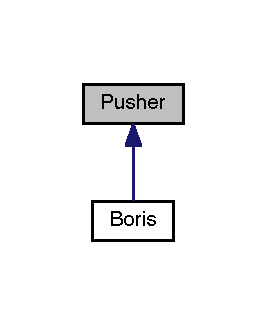
\includegraphics[width=128pt]{class_pusher__inherit__graph}
\end{center}
\end{figure}
\subsection*{Public Member Functions}
\begin{DoxyCompactItemize}
\item 
\hypertarget{class_pusher_a8a9a5faace14e07e8b42fb51cc83088e}{}\label{class_pusher_a8a9a5faace14e07e8b42fb51cc83088e} 
virtual int {\bfseries Step} (\hyperlink{struct_particle}{Particle} $\ast$part, \hyperlink{struct_field__part}{Field\+\_\+part} $\ast$field, double dt)=0
\end{DoxyCompactItemize}


The documentation for this class was generated from the following file\+:\begin{DoxyCompactItemize}
\item 
src/pusher/pusher.\+hpp\end{DoxyCompactItemize}

%--- End generated contents ---

% Index
\backmatter
\newpage
\phantomsection
\clearemptydoublepage
\addcontentsline{toc}{chapter}{Index}
\printindex

\end{document}
